\documentclass[11pt]{article}
\usepackage{listings}
\usepackage{graphicx}

\begin{document}

\setlength{\parindent}{0pt}

\section{File Structure}

In this section, the content of each folder is clarified.

\subparagraph{src}
Contains the code for the GLM parser. The structure of the src folder would be covered in the code structure section.

\subparagraph{scripts}
Contains the scripts for experiments. Such as the scripts to submit jobs in cluster, etc.

\subparagraph{logs}
Contains the experiments output and results. It is ordered based on the experiment date.

\subparagraph{docs}
Contains the documentation files.



\section{Code Structure}

In this section, the structure of the code in src folder. The project contains six modules to implement the GLM parser, backend, data, evaluate, feature, learn and parse. The functionality of each module is covered in the following subsections.

\subparagraph{data}

This module contains the classes used to load test data from Penn Treebank and creates the class DependencyTree which stores the information of test data (i.e. wordlist, taglist, edges in the dependency tree).

\subparagraph{feature}

This module contains the classes deal with features, such as extracting features from tagged sentences and holding the weight information of the features. The detailed class definitions is discussed in the Major Data Structure section.

\subparagraph{parse}

This module contains the parsing algorithm for the parser, such as eisner algorithm and eisner algorithm with second order, etc. 

The alternative parsers can easily substitute each other as long as they have the function: 
	$$ parse(sentence, score\_function) $$

\subparagraph{learn}

This module contains the learning algorithm for the GLM parser, such as perceptron, average perceptron and MIMA, etc. 

The alternative learners can easily substitute each other as long as they contains function: 
	$$ learn(feature\_set, current\_global\_vector, gold\_global\_vector) $$

\subparagraph{evaluate}

This module contains the evaluating algorithm. The evaluator takes the test data and the currently used parser, and calculates the accuracy for the parser. The accuracy used now is the dependency accuracy.

To add more accuracy test, you can either create alternative evaluators or add functions inside the evaluator. The alternative or modified evaluator should have function:
	$$ evaluate(data\_pool, parser, feature\_set) $$

\subparagraph{backend}

This module works with feature module to output the weight result into files using pickle.

The structure of the code makes the parser scalable in both parsing and learning. The summery of the project struct is shown in the following figure:

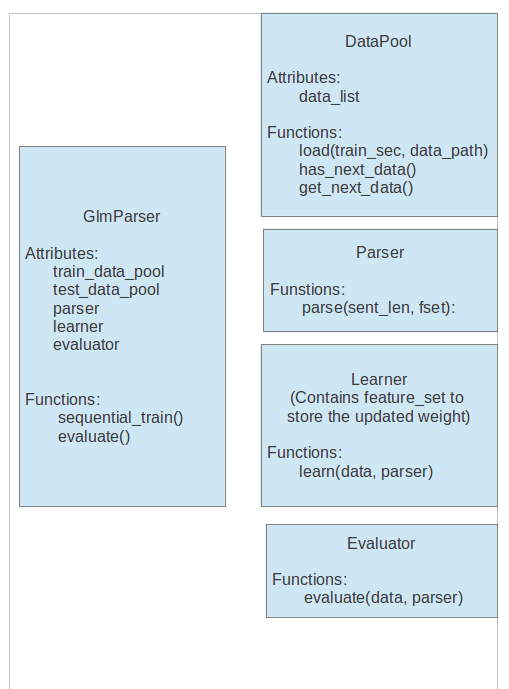
\includegraphics[scale=0.8]{project_struct}



\section{Major Data Structure}

This section explains the major classes in the project,

\subparagraph{DependencyTree}
A data structure that represents the result of a dependency parser. Each class instance stores four types of information. These information are: node set, POS set, edge set and edge type. Users could construct a dependency tree through these information. This class also provides interfaces to manipulate the information, including retriving nodes, edges, types, modifying nodes, edges, types, and other relevant tasks.

\subparagraph{FeatureSet}
Stores and updates weight vector used in dependency parsing according to
various features

\subparagraph{DataPool}
A data structure that stores the test data in a list of DependencyTree

\subparagraph{FeatureVector}
Stores the features of an edge in a dictionary.


\section{Feature Used}

The feature used in the project is as follows: \\

% TODO: formating

Unigram Features: \\

\begin{tabular}{|l|}
	\hline
		$xi-word, xi-pos$ \\
		$xi-word$ \\
		$xi-pos$ \\
		$xj-word, xj-pos$ \\
		$xj-word$ \\
		$xj-pos$ \\
	\hline
\end{tabular} \\




Bigram Features: \\

\begin{tabular}{|l| }
	\hline
		$xi-word, xi-pos, xj-word, xj-pos$ \\
		$xi-pos, xj-word, xj-pos$ \\
		$xi-word, xj-word, xj-pos$ \\
		$xi-word, xi-pos, xj-pos$ \\
		$xi-word, xi-pos, xj-word$ \\
		$xi-word, xj-word$ \\
		$xi-pos, xj-pos$ \\
	\hline
\end{tabular} \\



In-between Features: \\

\begin{tabular}{|l|}
	\hline
		$xi-pos, xb-pos, xj-pos$ \\
	\hline
\end{tabular} \\



Surrounding Features: \\

\begin{tabular}{|l| p{10cm} |}
	\hline
		$xi\_pos, xi+1\_pos, xj-1\_pos, xj\_pos$ \\
		$xi\_pos, xi+1\_pos,          xj\_pos$ \\
		$xi\_pos,          xj-1\_pos, xj\_pos$ \\
		$xi-1\_pos, xi\_pos, xj-1\_pos, xj\_pos$ \\
		$         xi\_pos, xj-1\_pos, xj\_pos$ \\
		$xi-1\_pos, xi\_pos,          xj\_pos$ \\
		$xi\_pos,          xj\_pos, xj+1\_pos$ \\
		$xi\_pos, xi+1\_pos, xj\_pos         $ \\
		$xi-1\_pos, xi\_pos, xj\_pos, xj+1\_pos$ \\
		$         xi\_pos, xj\_pos, xj+1\_pos$ \\
		$xi-1\_pos, xi\_pos, xj\_pos         $ \\
	\hline
\end{tabular} \\
            


\section{Algorithms Implemented}

\subparagraph{Parse}
Eisner, ...

\subparagraph{Learn}
Perceptron, ...

\subparagraph{evaluate}
Dependency Accuracy, ...


\end{document}